% Magic comment to tell latex to compile with lualatex
% !TeX program = lualatex

\documentclass[11pt,a4paper]{article}

\usepackage{indentfirst}
\usepackage{shellesc,xpatch}
\usepackage[french]{translator}
\usepackage{float}
\usepackage{glossaries} % Pour faire des glossaires
\usepackage{natbib} % Pour créer des références bibliographiques
\usepackage{comment} % Pour les commentaires
\usepackage{graphicx} % Pour les images
\usepackage[francais]{babel} % Document FR
\usepackage[T1]{fontenc} % Document FR
\usepackage{fontspec} 
\usepackage{fancyhdr} % Pour des en-tête et pied de page stylé
\usepackage{url} % Pour afficher les URL
\usepackage{appendix} % Pour les annexes
\usepackage{listings} % Pour les tables de code.
\usepackage{eso-pic}
\usepackage{wrapfig}
\usepackage{todonotes} % Pour les TODO
\usepackage{xcolor} 
\usepackage[cache=false]{minted} % Pour afficher du code proprement. Besoin de rajouter cache=false pour corriger un bug dans minted
\usepackage[normalem]{ulem} 
\usepackage{enumerate} % Des listes numérotées.

\usepackage{lipsum} % only for demonstrating purpose, you can safely remove this package
%% \lipsum
%% \lipsum[3-56] 

\usepackage{tikz}
\usetikzlibrary{calendar}
\usepackage{placeins}
\usepackage{textcomp}
\usepackage{pgfgantt}

% Définitions des titres
\renewcommand\listoflistingscaption{Liste des codes sources}
\renewcommand\listingscaption{Code}

% pour switch auto papier / pdf
\newtoggle{paper}

% Pick one and comment the other one.
% \toggletrue{paper}
\togglefalse{paper}

\iftoggle{paper}{%
	% paper
	\usepackage[left=3cm,right=2cm,top=2cm,bottom=2cm]{geometry} % Pour le rapport imprimé   
}{%
	% electronic
	\usepackage[left=3cm,right=3cm,top=3cm,bottom=3cm]{geometry}
}

% Gestion des marges. Lien utile.
% https://www.debian-fr.org/t/latex-definir-un-paragraphe-en-dehors-des-marges/13991/3

% Réglages d'affichage
\setcounter{tocdepth}{2} % granularité de la table des matières
\setlength{\parindent}{3em} % On modifie l'indentation des paragraphes
\setlength{\parskip}{1em} % On modifie l'espace entre les paragraphes
\widowpenalty=10000 % Pour les veuves et les orphelines
\clubpenalty=10000 % Pour les veuves et les orphelines
\FrenchFootnotes %% FROM : http://www.xm1math.net/doculatex/notesbasdepage.html
\newcommand{\numerotationType}{arabic} %Type de numérotation : Roman ou arabic

%% FROM http://forum.mathematex.net/latex-f6/glossaire-t8654.html#p85429
\renewcommand{\glstextformat}[1]{#1*} % Affichage dans le corps du texte d'une entrée du glossaire
%%%%%%%%%%%%%%%%%%%%%%%%%%%%%%%%%%%%%%%%%%%%%%%%%%%%%%%%%%%%%%%%%%%%%%%%%%%%%%%%%%%%%%%%%%%%%%
\begin{comment}
	Fonction utilisée pour insérer une image. L'image doit être située dans le répertoire "img"
	Paramètres : 
	#1 : Positionnement de l'image [Paramètre optionnel]
			H 	Place le flottant ici, c'est-à-dire à l'endroit auquel il apparaît dans le texte source.
			t 	Position en haut de la page.
			b 	Position en bas de la page.
			p 	Place sur une page particulière réservée aux flottants.
			! 	Passe outre les paramètres internes que Latex utilise pour déterminer une position optimale des flottants. (déconseillé)
	#2 : échelle de l'image
	#3 : nom absolu du fichier (extension du fichier comprise)
	#4 : Commentaire affiché sous l'image
	#5 : id de l'image (utile pour y faire référence par la suite)
	Exemple d'utilisation :
	\newImage{2}{test.png}{ceci est un test}{test} : Laisser LateX se demerder pour placer au mieux
	\newImage[H]{2}{test.png}{ceci est un test}{test} : Forcer le placement de l'image à cet endroit exact.
\end{comment}
\newcommand{\newImage}[5][h]
{
\begin{figure}[#1]
    \centering
    \includegraphics[scale=#2]{img/#3}
    \caption{#4}
    \label{fig:#5}
\end{figure}
}

%%%%%%%%%%%%%%%%%%%%%%%%%%%%%%%%%%%%%%%%%%%%%%%%%%%%%%%%%%%%%%%%%%%%%%%%%%%%%%%
% Same as before, but annexe without captions.
\newcommand{\newImageAnnexe}[4][h]
{
\begin{figure}[#1]
    \centering
    \includegraphics[scale=#2]{img/#3}
    \label{annexe:#4}
\end{figure}
}

%%%%%%%%%%%%%%%%%%%%%%%%%%%%%%%%%%%%%%%%%%%%%%%%%%%%%%%%%%%%%%%%%%%%%%%%%%%%
\begin{comment}
	Fonction utilisée pour ajouter une URL.
	@see http://timmurphy.org/2010/04/04/referencing-website-urls-with-latex-bibtex/ ?
	Paramètres : 
	#1 : url (doit OBLIGATOIREMENT faire référence à un id de main.bib)
	#2 : Nom donné
	Exemple d'utilisation :
	\addURL{www.google.fr}{Google}
\end{comment}
\newcommand{\addURL}[2]
{
#2\footnote{#1 (cf. entrée \cite{#1} des références)}
}

%%%%%%%%%%%%%%%%%%%%%%%%%%%%%%%%%%%%%%%%%%%%%%%%%%%%%%%%%%%%%%%%%%%%%%%%%%%%%
\begin{comment}
	Fonction pour ajouter un acronyme contenant une définition au glossaire.
	Paramètres : 
	#1 : id acronyme
	#2 : Nom acronyme court
	#3 : Nom complet acronyme
	#4 : Description dans le glossaire

	Exemple d'utilisation :
	\newAcronym{API}{API}{Application Programming Interface}{Définition de API}
\end{comment}
\newcommand{\newAcronym}[4]
{
	\newglossaryentry{#1}
	{
			name={#2},
			description={#4},
			first={\glsentrylong{#1} (#2)},
			long={#3}
	}
}

%%%%%%%%%%%%%%%%%%%%%%%%%%%%%%%%%%%%%%%%%%%%%%%%%%%%%%%%%%%%%%%%%%%%%%%%%%%%%%%%%%%%%%%%%%%%%%
% http://www.developpez.net/forums/d961640/autres-langages/autres-langages/latex/mise-forme/referencer-annexe/#post5400726
% Pas un grand intérêt, mais à garder sous le coude, on sait jamais.
\newcommand{\annexe}[1]{annexe~\ref{#1} (page~\pageref{#1})}
%%%%%%%%%%%%%%%%%%%%%%%%%%%%%%%%%%%%%%%%%%%%%%%%%%%%%%%%%%%%%%%%%%%%%%%%%%%%%%%%%%%%%%%%%%%%%%
\begin{comment}
	Quelques commandes utiles pour la compilation avec un index ou des références.
	
	Build Glossaries
		- "makeindex.exe -s main.ist -t main.glg -o main.gls main.glo"
	
	Build References
	- "bibtex main"
	
	Exemple bibliographie dans le fichier main.bib :
	\@Misc{ 
		google, % Identifiant pour y faire références
		note = {}, % Une note optionnelle
		title = {Google}, % Titre
		author = {\url{google.com}} % Lien vers URL ou titre du livre.
	}
	
	Créer des tableaux LateX facilement
	http://www.tablesgenerator.com
	
\end{comment}

%%%%%%%%%%%%%%%%%%%%%%%%%%%%%%%%%%%%%%%%%%%%%%%%%%%%%%%%%%%%%%%%%%%%%%%%%%%%%%%%%%%%%%%%%
% This is where the magic happens..
\newcommand{\nocontentsline}[3]{}
\newcommand{\tocless}[2]{\bgroup\let\addcontentsline=\nocontentsline#1{#2}\egroup}

% Définir le titre des annexes dans le sommaire (ne marche pas si mis dans parameters)
\renewcommand{\addappheadtotoc}{Annexes}

% Création glossaire
\makeglossaries
% Chargements des entrées du glossaire. APRES \makeglossaries
\loadglsentries{glossaire.tex}

% Début du document
\begin{document}	
	\pagestyle{plain} % Juste le numero de page pour en-tête / pied de page.
	\pagenumbering{gobble} % pas de numérotation
	%%%%%%%%%%%%%%%%%%%%%%%%%%%%%%%%%%%%%%%%%
% University Assignment Title Page 
% LaTeX Template
% Version 1.0 (27/12/12)
%
% This template has been downloaded from:
% http://www.LaTeXTemplates.com
%
% Original author:
% WikiBooks (http://en.wikibooks.org/wiki/LaTeX/Title_Creation)
%
% License:
%% CC BY-NC-SA 3.0 (http://creativecommons.org/licenses/by-nc-sa/3.0/)
% 
% Instructions for using this template:
% This title page is capable of being compiled as is. This is not useful for 
% including it in another document. To do this, you have two options: 
%
% 1) Copy/paste everything between \begin{document} and \end{document} 
% starting at \begin{titlepage} and paste this into another LaTeX file where you 
% want your title page.
%% OR
% 2) Remove everything outside the \begin{titlepage} and \end{titlepage} and 
% move this file to the same directory as the LaTeX file you wish to add it to. 
% Then add \input{./title_page_1.tex} to your LaTeX file where you want your
% title page.
%
%%%%%%%%%%%%%%%%%%%%%%%%%%%%%%%%%%%%%%%%%

\begin{titlepage}

\newcommand{\HRule}{\rule{\linewidth}{0.5mm}} % Defines a new command for the horizontal lines, change thickness here

\center % Center everything on the page
 
%----------------------------------------------------------------------------------------
%%	HEADING SECTIONS
%----------------------------------------------------------------------------------------

\textsc{\LARGE University Name}\\[1.5cm] % Name of your university/college
\textsc{\Large Department Name}\\[0.5cm] % Major heading such as course name
\textsc{\large Formation Name}\\[0.5cm] % Minor heading such as course title
\space
%----------------------------------------------------------------------------------------
%%	TITLE SECTION
%----------------------------------------------------------------------------------------

\HRule \\[0.4cm]
{ \huge \bfseries Title}\\[0.4cm] % Title of your document
\HRule \\[1.5cm]

\begin{minipage}{0.4\textwidth}
\begin{flushleft} \large
\emph{Enterprise tutor :}\\
Firstname \textsc{NAME} % Tutor's name
\end{flushleft}
\end{minipage}
~
\begin{minipage}{0.4\textwidth}
\begin{flushright} \large
\emph{Internship director:} \\
Firstname \textsc{name} % Supervisor's Name
\end{flushright}
\end{minipage}\\[2cm]

\Large \emph{Student :}\\
Firstname \textsc{name}\\[3cm] % Your name

{\large \today}\\[2cm] % Date, change the \today to a set date if you want to be precise

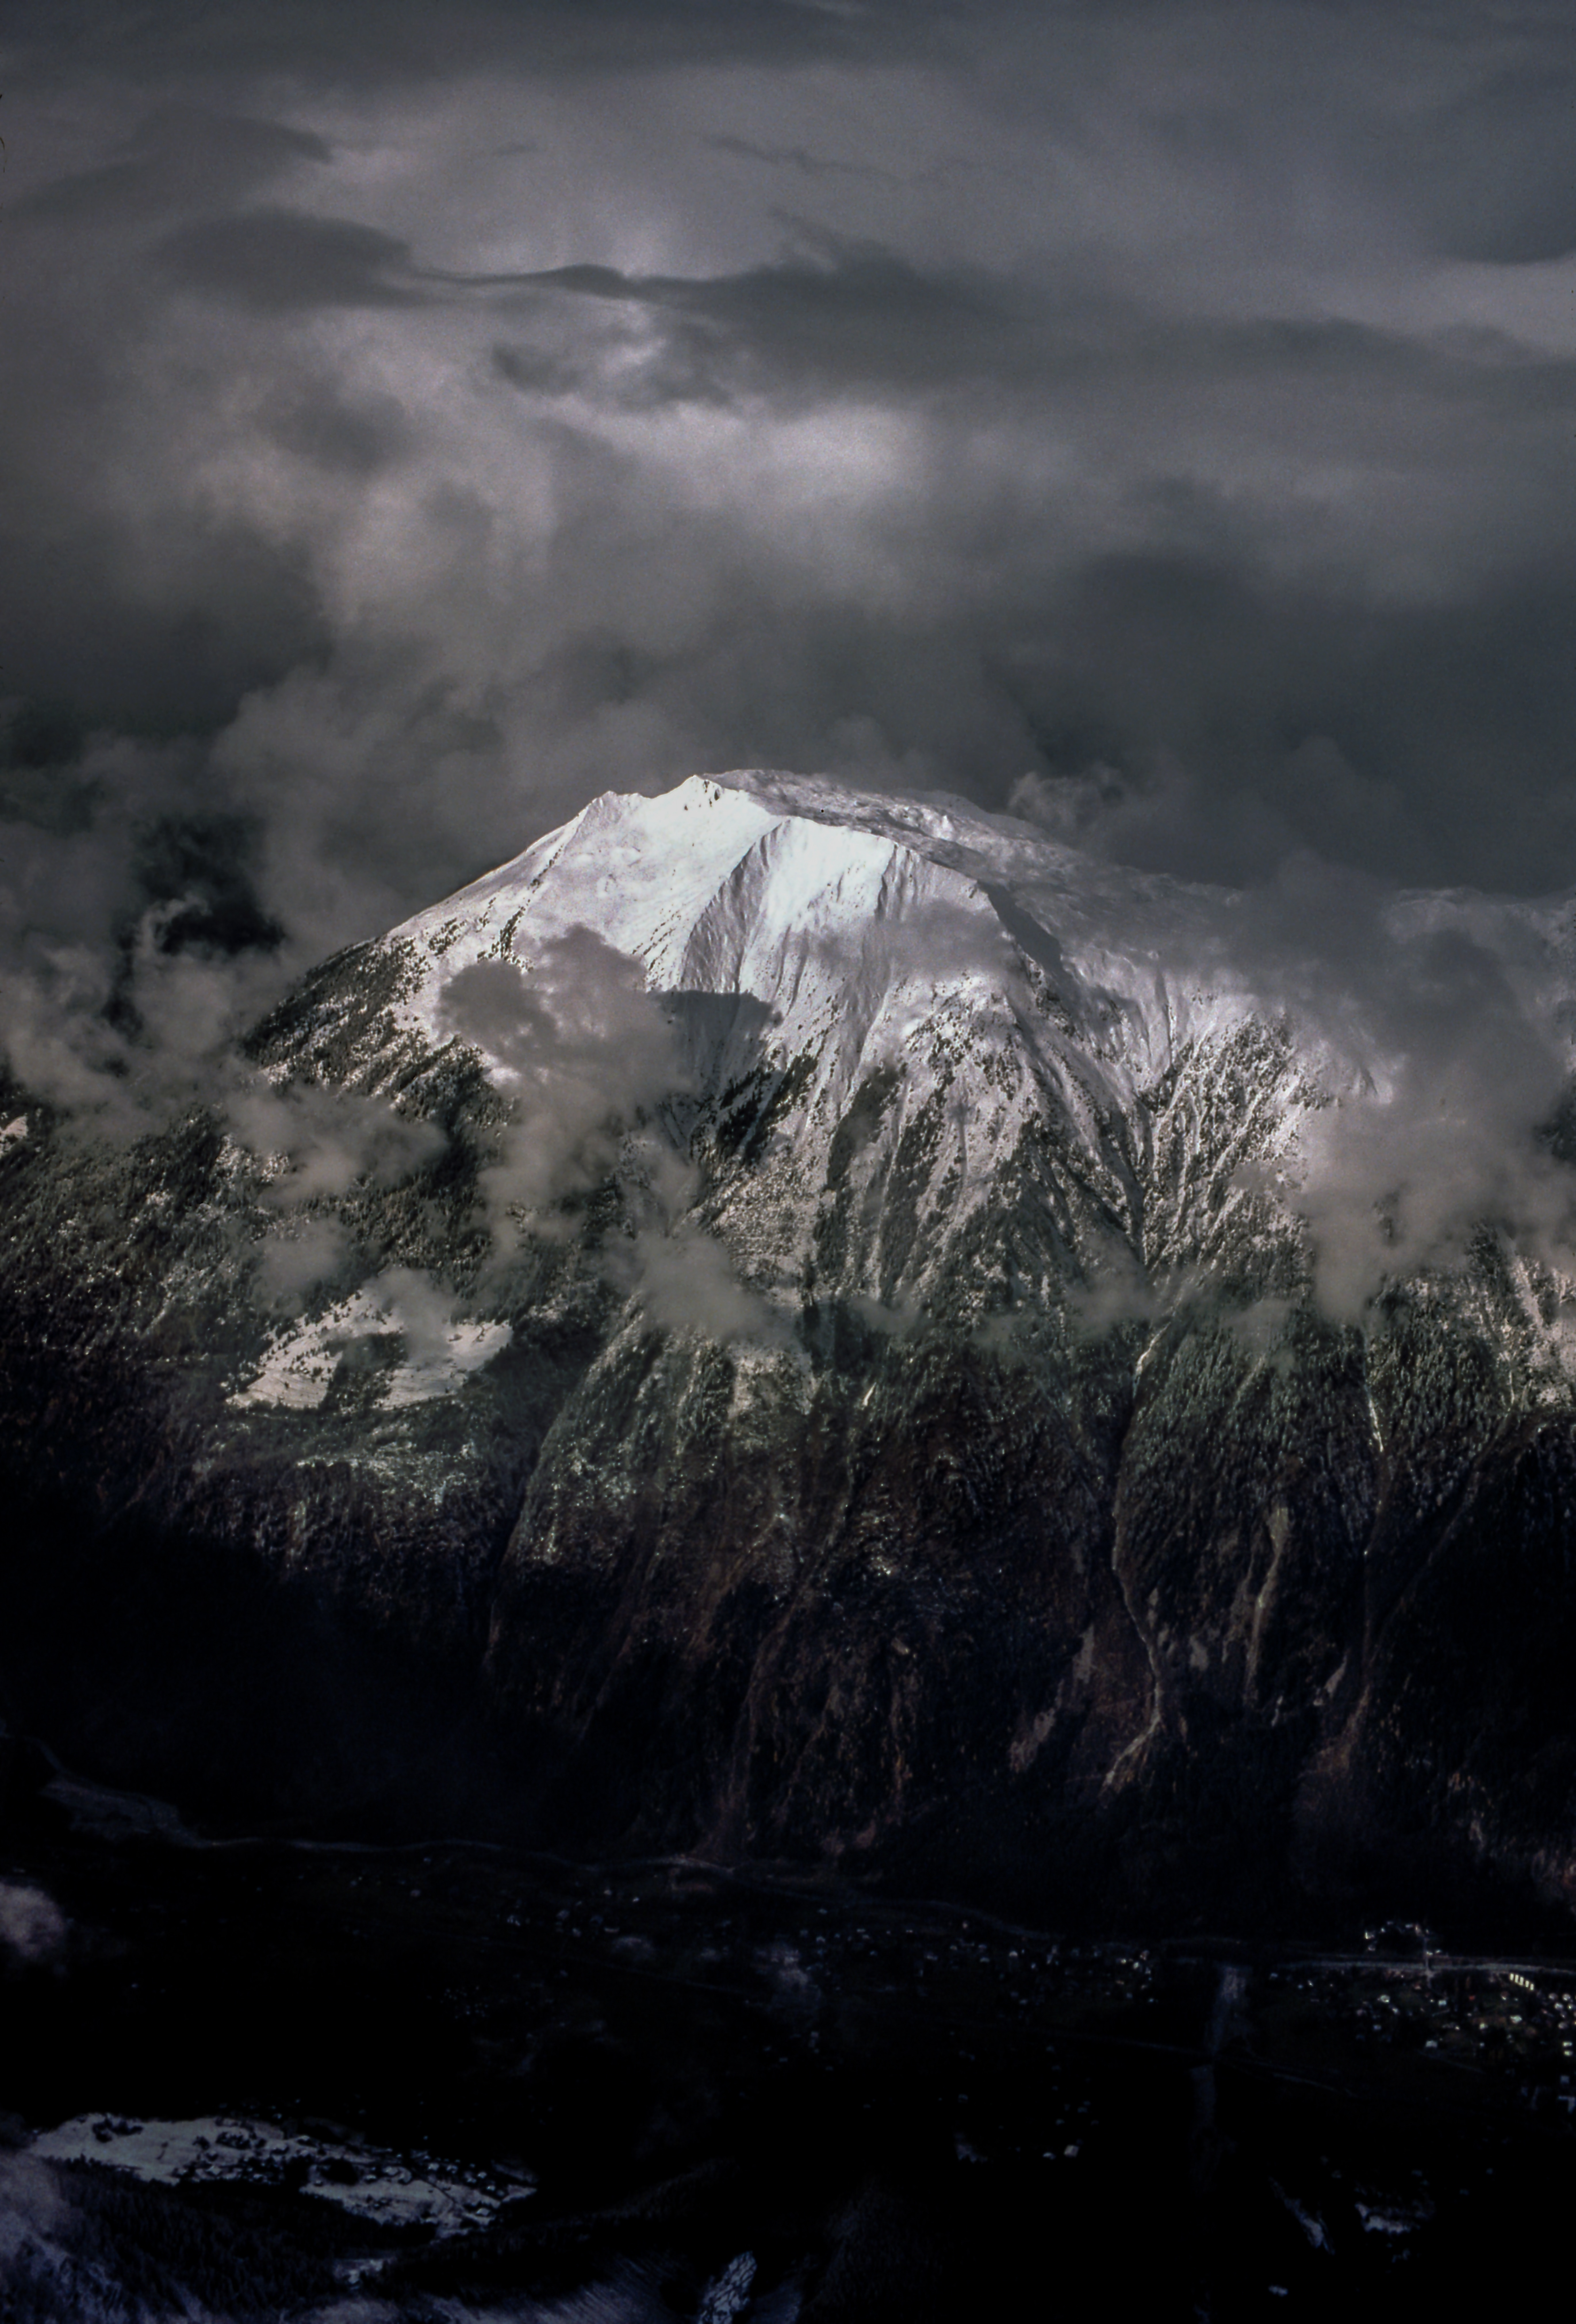
\includegraphics[scale=0.02]{img/image.jpg}\\[1cm] % Include a department/university logo - this will require the graphicx package
 
\vfill % Fill the rest of the page with whitespace

\end{titlepage} 
	
\newpage
	~ % Hide thanks page.
\newpage
	%% TODO Listing. Comment this page before printing !
	\listoftodos 
\newpage
	% \section* mean unnumeroted section
  \section*{Thanks page.}
	\vfill

\todo{Reminder to tell me to add something here later}
\lipsum[5]

\vfill
\newpage
	% Define Sommaire instead of "Table of Content"
	\renewcommand{\contentsname}{Sommaire}
	\tableofcontents
\newpage
	\pagenumbering{\numerotationType} % start numerotation
	\section*{Introduction}
	\addcontentsline{toc}{section}{Introduction} % ajout de la référence dans la table des matières
	\vfill
	\macOS{} command is used. 
	\missingfigure{A missing figure that I'll add later}
\vfill
\newpage
	%%%%%%%%%%%%%%%% FANCY %%%%%%%%%%%%%%%%%
	% Fancy header / footer
	\pagestyle{fancy}
	
	% Obtenir le nom de la section/sous-section sans le numero
	\renewcommand{\sectionmark}[1]{\markright{#1}}
	\renewcommand{\subsectionmark}[1]{\markright{#1}}
	\renewcommand{\subsubsectionmark}[1]{\markright{#1}}
	
	%% HEADER
	%\renewcommand{\headrulewidth}{0.4pt}
	\lhead{\fancyplain{}{}}
	\chead{\fancyplain{}}
	\rhead{\fancyplain{}{\rightmark}}
	
	%% FOOTER
	%\renewcommand{\footrulewidth}{0.4pt}
	\lfoot{\fancyplain{}{}}	
	\cfoot{\fancyplain{}{}}	
	\rfoot{\fancyplain{}{\thepage}}
	%%%%%%%%%%%%%%%% END FANCY %%%%%%%%%%%%

  \section{Context}
	\subsection{Subsection example}
	\lipsum[2]
\subsubsection{Subsubsection example}

	\lipsum[2]
	\begin{itemize}
		\item \lipsum[2]
		\item \lipsum[2]
	\end{itemize}
\clearpage
\newpage
	\section{Main Content}
	\subsection{Project presentation}
	Table example : 

% Créer des tableaux LateX facilement
% http://www.tablesgenerator.com
\begin{table}[H] % Le paramètre H (majuscule) signifie : place cet élément à cet endroit précisement.
\centering
\begin{tabular}{|c|l|l|l|}
\hline
\textbf{Utilisateur} & \multicolumn{1}{c|}{\textbf{Version 1}} & \multicolumn{1}{c|}{\textbf{Version 2}} & \multicolumn{1}{c|}{\textbf{Version 3}} \\ \hline
\textit{Pierre} & Non & Non & Oui \\ \hline
\textit{Paul} & Oui & Oui & Non \\ \hline
\textit{Jacques} & Oui & Oui & Non \\ \hline
\textit{Hector} & Oui & Oui & Oui \\ \hline
\end{tabular}
\caption{Accès des différents utilisateurs aux différents versions}
\label{tab:versions}
\end{table}
\subsubsection{Task 1}
	\lipsum

\newImage[H]{0.05}{image.jpg}{Image example}{image-example}
s
\begin{itemize}
	\item \lipsum[5]
	\item \lipsum[5]
	\item \lipsum[5]
\end{itemize}


\begin{enumerate}
	\item \lipsum[4]
	\item \lipsum[4]
\end{enumerate}

\paragraph*{Reference to annexes, bibliography URL \& Glossary items}

	Hello (cf. annexe \ref{code:php-example})
	
	Here is a link example \addURL{http://google.com}{My custom Text}.
	
	Acronym example : \gls{HTML}

\subsubsection{Task 2}
	\lipsum[12-13]

\begin{listing}[H]
	\caption{Example of PHP Code}
	\inputminted[breaklines,linenos]{php}{code/entity.php}
	\label{code:entity}
\end{listing}


\begin{listing}[H]
	\caption{Exemple Markdown}
	\inputminted[breaklines,linenos]{php}{code/markdown.md}
	\label{code:markdown}
\end{listing}
\clearpage
\newpage
	\pagestyle{plain} % Juste le numero de page pour en-tête / pied de page à partir de maintenant
	\section*{Conclusion}
	\addcontentsline{toc}{section}{Conclusion} % ajout de la référence dans la table des matières
	
\vfill

\lipsum[4-5]
\vfill
\newpage
	\addcontentsline{toc}{section}{Glossaire, références, tables des codes, des figures, des tableaux et annexes}
	\glsaddall % ajouter toutes les entrées n'ayant pas encore été citées
  \printglossaries % afficher le glossaire
\newpage	
	\nocite{*} % Add all bibliography items that have not been listed yet.
	\bibliographystyle{unsrt} 
	\bibliography{main}{}
	\clearpage

	\listoffigures 
	\listoflistings
	\listoftables
\newpage
	\pagenumbering{gobble} % No numerotation
	\vspace*{\stretch{1}}
		\begin{center}
			\begin{Huge}
				\section*{\MakeUppercase{Annexes}} 
			\end{Huge}
		\end{center}
	\vspace*{\stretch{1}}
\newpage
	\appendix % Annexes with A, B, C, D numerotation
	\section{Image in Annexes}
	\newImageAnnexe[!t]{0.05}{image.jpg}{An image in Annexes}
	\newpage
\section{Code example from PHP Sample file}
	\begin{listing}[H]
	    \inputminted[breaklines,linenos]{php}{code/ppt.php}
	    \label{code:php-example}
    \end{listing}
\section{Gantt du travail réalisé}
	\def\pgfcalendarweekdayletter#1{

\ifcase#1L\or M\or M\or J\or V\or S\or D\fi
}
\ganttset{
%
calendar week text={
%
\startday~\pgfcalendarmonthshortname{\startmonth}~\startyear
%
}
%
}
\shorthandoff{:!}
\noindent\resizebox{\textwidth}{!}{
    
    \begin{ganttchart}[
        hgrid,
        vgrid,
        x unit=4mm,
            group label font=\tiny,
            title label font=\small,
            y unit chart = 1cm,
            y unit title = 0.8cm,
            bar/.append style={fill=blue!20},
            milestone/.append style={fill=red!70},
        time slot format=little-endian
        ]{04/04/2016}{10/06/2016}
        
        \gantttitlecalendar{week=1, weekday=letter} \\
				
				%% NEXT
				\ganttbar{0}{04/04/2016}{06/04/2016}\\
				\ganttbar{1}{06/04/2016}{07/04/2016}\\
				\ganttbar{2}{07/04/2016}{11/04/2016}\\
				\ganttbar{3}{11/04/2016}{15/04/2016}\\
				\ganttbar{4}{06/06/2016}{06/06/2016}\\
				\ganttbar{5}{07/06/2016}{07/06/2016}\\
				
				%% LINK NEXT
				\ganttlink{elem0}{elem1}
				\ganttlink{elem1}{elem2}
				\ganttlink{elem2}{elem3}
				
				%% QUIZZBOX
				\ganttbar{6}{18/04/2016}{18/04/2016}\\
				\ganttbar{7}{19/04/2016}{19/04/2016}\\
				\ganttbar{8}{20/04/2016}{22/04/2016}\\
				
				%% LINK QUIZZBOX
				\ganttlink{elem6}{elem7}
				\ganttlink{elem7}{elem8}
				
				%% QB
				\ganttbar{9}{25/04/2016}{27/04/2016}\\
				\ganttbar{10}{27/04/2016}{29/04/2016}\\
				\ganttbar{11}{02/05/2016}{03/05/2016}\\
				\ganttbar{12}{03/05/2016}{04/05/2016}\\
				\ganttbar{13}{09/05/2016}{11/05/2016}\\
				\ganttbar{14}{12/05/2016}{13/05/2016}\\
				\ganttbar{15}{17/05/2016}{18/05/2016}\\
				\ganttbar{16}{17/05/2016}{19/05/2016}\\
				\ganttbar{17}{19/05/2016}{20/05/2016}\\
				\ganttmilestone{18}{20/05/2016}\\
				\ganttbar{19}{23/05/2016}{24/05/2016}\\
				\ganttbar{20}{25/05/2016}{26/05/2016}\\
				\ganttbar{21}{27/05/2016}{01/06/2016}\\
				\ganttbar{22}{01/06/2016}{03/06/2016}\\
				\ganttbar{23}{08/06/2016}{09/06/2016}\\
				%% LINK QB
				\ganttlink{elem9}{elem10}
				\ganttlink{elem10}{elem11}
				\ganttlink{elem11}{elem12}
				\ganttlink{elem12}{elem13}
				\ganttlink{elem13}{elem14}
				\ganttlink{elem14}{elem15}
				\ganttlink{elem15}{elem16}
				\ganttlink{elem16}{elem17}
				\ganttlink{elem17}{elem18}
				\ganttlink{elem18}{elem19}
				\ganttlink{elem19}{elem20}
				\ganttlink{elem20}{elem21}
				\ganttlink{elem21}{elem22}
				
				\ganttlink{elem22}{elem4}
				\ganttlink{elem4}{elem5}
				\ganttlink{elem5}{elem23}
				\ganttlink{elem3}{elem6}
				\ganttlink{elem8}{elem9}
        
    \end{ganttchart}
}

\begin{table}[]
\centering
\begin{tabular}{|l|l|}
\hline
0 & Formation Symfony2 \\ \hline
\multicolumn{2}{|c|}{\textbf{Refonte Nextmedia partie Administration}} \\ \hline
1 & Scroll Analytics \\ \hline
2 & Refonte graphique \\ \hline
3 & Gestion AJAX \\ \hline
4 & Déploiement Capistrano \\ \hline
5 & Ajout interface web de traduction \\ \hline
\multicolumn{2}{|c|}{\textbf{Analyse QuizzBox MacOS}} \\ \hline
6 & Découverte application \\ \hline
7 & Recoupement des variables \\ \hline
8 & Etablissement des règles de gestion \\ \hline
\multicolumn{2}{|c|}{\textbf{Développement QBStore}} \\ \hline
9 & Gestion des téléchargements \\ \hline
10 & Ajout historique \\ \hline
11 & Filtres questionnaires \\ \hline
12 & Champ de recherche page version \\ \hline
13 & Version de démonstration \\ \hline
14 & Récupération utilisateurs depuis Access \\ \hline
15 & Mail template POC \\ \hline
16 & Implémentation Mail Template \\ \hline
17 & Correction de bugs \\ \hline
18 & Réunion mi parcours \\ \hline
19 & Capistrano \\ \hline
20 & Ajout WebService liaison Access \\ \hline
21 & Recherches façons optimale de traduire un site \\ \hline
22 & Implémentation de la solution : Interface de traduction web \\ \hline
23 & Inscription par domaine \\ \hline
\end{tabular}
\end{table}
\label{gantt}
	\newpage
\clearpage
\end{document}